\chapterimage{street_plaque.jpg}

\chapter{Where are you?}\label{sec:where}

Connecting two computers makes them much more useful than two isolated machines. 
However, their true potential is only unlocked when they can be connected to \textit{lots} of other computers.

Practical limitations including cost and geographic location make it impossible to directly
connect every pair of computers. Instead, devices are distributed across a graph of interconnected networks,
which may extend even beyond the scale of a planet.

Whether locally within physical reach or in another continent, an addressing system is needed
to identify, locate and route messages so that they reach their intended peers, just like we 
do with physical locations.



\section{Please contact me}\label{sec:where:topology}

When only $2$ \conceptRef{device}{devices} are involved, one may use a \concept{point-to-point} connection. In this type of connection,
there is only ``this side'' and ``the other side'' of the cable. Moreover, when a device wants to communicate with the other end, 
there is only one link (\eg, one cable) to choose from, so there is no possible confusion. Since we can operate this connection 
with just $2$ \conceptRef{network card}{network cards} and $1$ cable, point-to-point connections are viable for $N=2$ devices.

\begin{wrapfigure}{R}{0.25\linewidth}
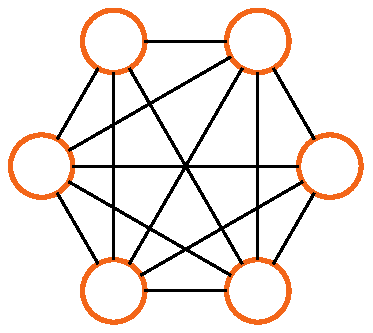
\includegraphics[width=\linewidth]{complete_graph.pdf}
\end{wrapfigure}


If we want to connect $N > 2$ devices, a naïve option is to connect every device with each other
in a \conceptRef{complete graph}{\textit{complete graph}}. Now every device needs to handle $N - 1$ cables to the other devices, 
but communicating with any other device is as easy as choosing the correct cable and establishing a point-to-point connection.

The main issue with this approach is that the total number of connections is $N \cdot (N-1) / 2 = O(N^2)$
(more on that in your trusted \textit{Discrete Math} course). This means that, in order to have $N=10$ devices connected in this way,
you would need for instance $40$ cables \textit{and} $90$ \conceptRef{network card}{network cards}. For $N=1000$ devices, 
there would be half a million point-to-point connections, which is already quite unmanageable.

\begin{remark}
$O(N^2)$ is notation for a \concept{quadratic} complexity bound. 
This is \textit{not} the same as \concept{exponential} and should never be confused.
% 
\readMore{https://en.wikipedia.org/wiki/Big_O_notation}
\end{remark}

\begin{wrapfigure}{L}{0.17\linewidth}
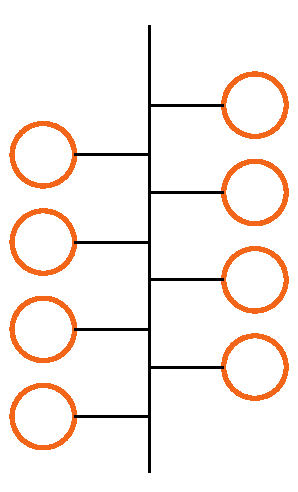
\includegraphics[height=4cm]{bus_graph.pdf}
\end{wrapfigure}

There is one trick up our sleeves: \conceptRef{bus}{data buses}, where one or more data lines
that are simultaneously connected to multiple devices. 
This retains the simplicity of point-to-point connections, because each device needs to handle
only $1$ cable and can use it to communicate with all other devices. The cost-effectiveness is 
also retained, since only $N$ network cards for $N$ devices ($O(N)$). 

The main advantage of data buses is also their main weakness: 
all devices send and receive data using the same data line, 
but they cannot do it at the same time because there is only one line. If two or more do, there is
a \concept{collision} that makes data transmission impossible while it lasts.\\[-0.5cm]

\begin{remark}
As computer networking was developed, people experimented with many alternatives to the 
bus \concept{topology}. One curious example is \concept{Token Ring}, where devices
are connected around a circle, and messages are passed around in a single direction.
\end{remark}

In practice, it is not trivial to implement a bus technology 
where new devices can be added over time. 
% 
Historically, this was sometimes done by physically piercing the main bus cable,
and adding a new cable towards the new computer being connected. 
Later on, this was simplified with devices called \conceptRef{hub}{hubs}. 
They worked similarly, but they offered pre-built \conceptRef{port (physical layer)}{ports} 
and removable connectors.
% 
Nowadays, hubs have been replaced by \conceptRef{switch}{switches}. 
Switches offer the functionality of a bus, connecting every device with each other,
and also prevent collisions. For obvious reasons, structuring connections 
around a switch is called a \concept{star topology}.

\begin{exercise}
What is \textbf{needed in a switch} that is not needed in a hub?

\begin{center}
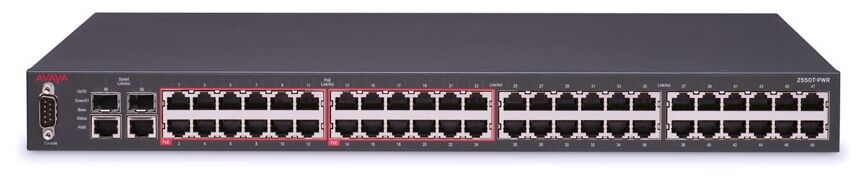
\includegraphics[width=0.75\linewidth]{switch.jpg}
\end{center}
\end{exercise}

Bus topologies work great at local scales, and are extensively employed in
\conceptRef{LAN}{local area \conceptRef{network}{networks} (LANs)}. However, it is not cost-effective,
(sometimes not even physically possible) when devices are far apart.
% 
Instead, devices can be organized in separate LANs, each one conceptually a bus, 
and then these separate LANs can be connected using cheaper, feasible point-to-point
connections. Considered together, these devices would then form a 
\conceptRef{WAN}{wide-area network (WAN)}.

\begin{center}
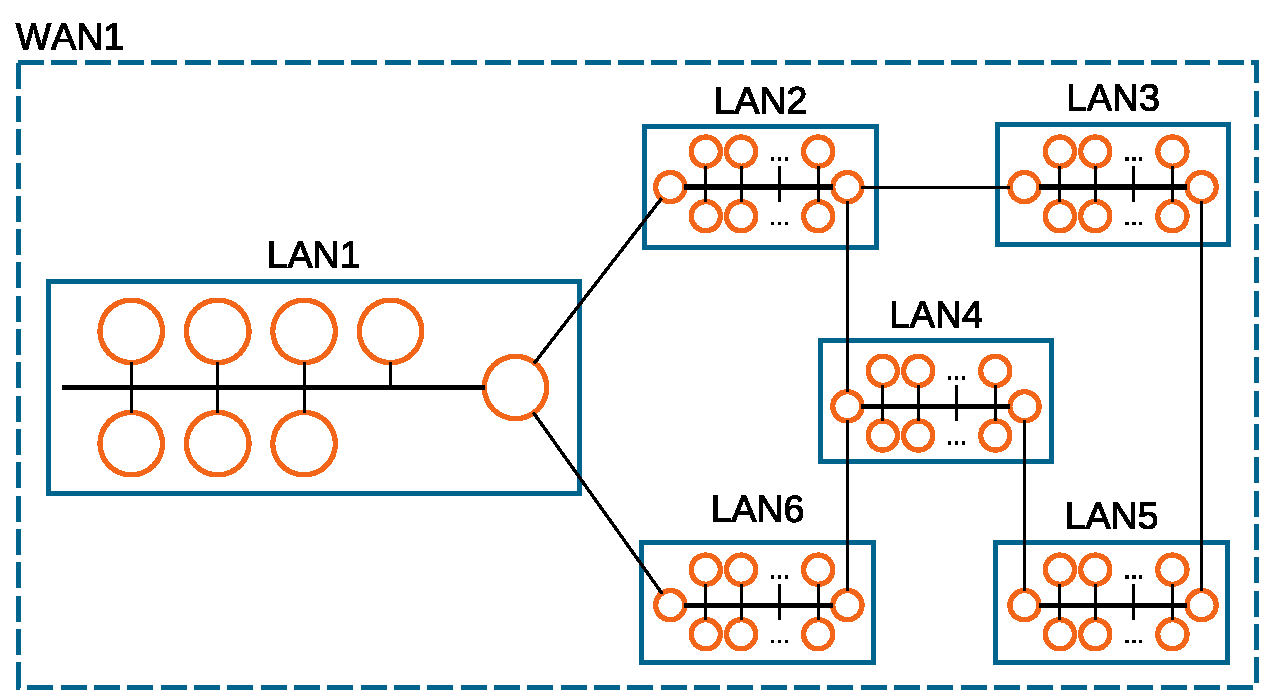
\includegraphics[width=0.65\linewidth]{lan_wan_structure.pdf}
\end{center}


\section{I need to find you}\label{sec:where:addresses}

Once again, the main advantage of data \conceptRef{bus}{buses} is also their main weakness: 
all devices send and receive data using the same data line. 
Even if collisions don't happen, every message sent into the bus is 
received by all devices.
However, what we actually want is for our message to reach its destination, 
and only its destination. Let's call this the \textit{find-my-device problem}.

The find-my-device problem is not unique of buses or \conceptRef{LAN}{LANs}. On the contrary, it becomes 
very important when we consider \conceptRef{WAN}{WANs}, where not all devices are directly interconnected.
In this case, we need to make sure we can \conceptRef{routing}{route} our messages
between different LANs, and that they reach their destination.

Surprisingly, not even point-to-point connections are safe from the find-my-device problem.
Assuming devices A and B are connected that way, two different programs may want to 
exchange information at the same time, \eg, some alarm control software and 
a music streaming app. 
In this scenario, you want the \concept{client} and \concept{server} of the alarm monitoring 
\concept{service} to communicate with each other but not with the music streaming service, 
and vice-versa.

The most common solution to this problem is to use identifiers that let
us differentiate between devices or even between running \conceptRef{process}{processes}
inside an \conceptRef{OS}{operating system (OS)}. Some of these identifiers are
referred to as \conceptRef{address}{addresses}, precisely because they are used 
to find and reach a remote device. 


\conceptRef{address}{Addresses} are typically \textit{numerical} identifiers, that is, just a number.
As such, they can be expressed in different bases, including decimal and \concept{hexadecimal}.
These numbers are drawn from a predefined set, and the choice of that set
determines the maximum number of elements we can uniquely identify.

\begin{remark}
Addresses expressed as \otherBase{d8:43:ae:61:ed:f1} or \otherBase{192.168.1.1} 
(as it will be seen later in the course) are also numbers we could have expressed 
as \otherBase{237785200061937} and \otherBase{3232235777}, respectively
(which is not as convenient).
\end{remark}

\begin{exercise}
\textbf{How many elements can be uniquely identify} (at most) with an address we express 
using 5 bits? How about 10? How about 20? Express the general solution mathematically.
\end{exercise}

\begin{exercise}
Suppose there are $1000$~machines in a LAN. \textbf{How many address bits are needed}?
How about $800$~machines? And $1100$? Express the general solution mathematically.
\end{exercise} 

\begin{remark}
In 2019, we run out of Internet (v4) addresses. Whoops!
\end{remark}

\section{How do I get there?}

In many scenarios, multiple addresses are needed to perform the desired 
\concept{end-to-end} communication. For instance, we may need to identify
a single device within a \concept{LAN}, and that LAN within a \concept{WAN}. Sometimes, we will need 
to identify a \concept{process} (a running program) within that device. 
This is not unlike someone paying you a visit in person:

\begin{minipage}{0.5\linewidth}
\begin{center}
\begin{bytefield}{16}
\bitbox{16}{Joseph Edgar Foreman} \\
\bitbox{16}{123 South Fake St.} \\
\bitbox{16}{Adams County} \\
\bitbox{16}{Ohio}
\end{bytefield}
\end{center}
\end{minipage}
% 
\begin{minipage}{0.5\linewidth}
\begin{center}
\begin{bytefield}{24}
\bitbox{24}{Process \#1717403} \\
\bitbox{24}{Device \#51688798} \\
\bitbox{24}{LAN 3141 (Data Engineering Labs)} \\
\bitbox{24}{WAN 442 (UAB)}
\end{bytefield} 
\end{center}
\end{minipage}

Whatever addressing system we use, it must contain enough information to locate and reach 
the destination, \ie, to \conceptRef{routing}{route} our messages through the graph of 
connections. The process of routing involves multiple steps or ``jumps'' across networks
until the destination LAN is reached.

The name \concept{router} refers to a type of network device
whose job is to forward these messages across networks. These devices must contain
enough information so that, when handed a message with a destination \concept{address},
they can decide what \concept{network interface} to use. 
In turn, non-router devices only need to be configured so that they can reach the next router.


\begin{remark}
At home, your \concept{router} typically also plays the role of a \concept{switch}, but those are different concepts.
\end{remark}

% \begin{center}
% 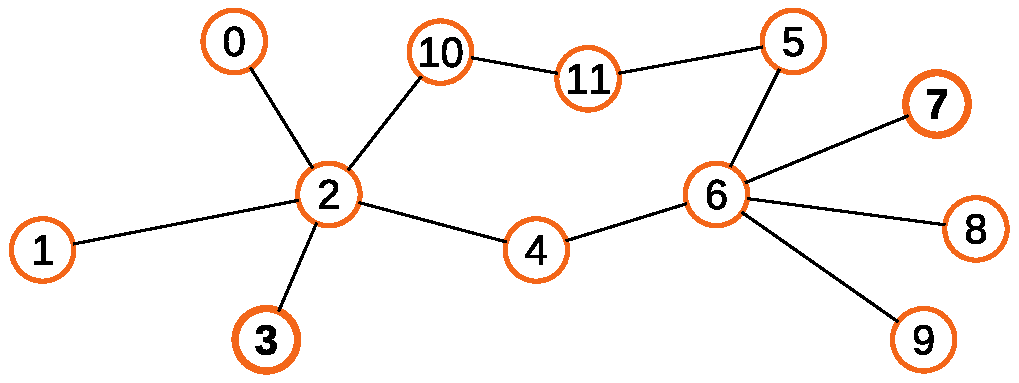
\includegraphics[width=0.5\linewidth]{how_many_packets.pdf}
% \end{center}

\begin{exercise}
This figure represents a handful of devices and their physical connections.
These devices can communicate only by sending messages through 
those connections. Notwithstanding, \node{3} wants to send a message to \node{7}.\\
% 
\begin{center}
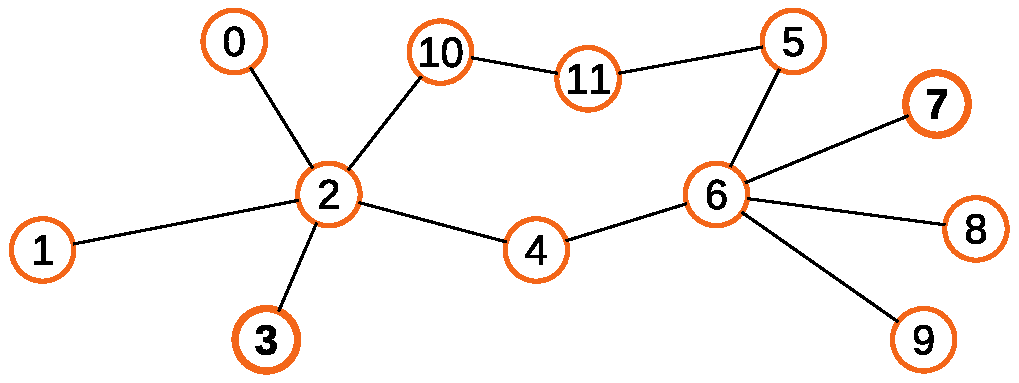
\includegraphics[width=0.5\linewidth]{how_many_packets.pdf}\\
\end{center}
% 
\begin{itemize}
 \item Can you identify any devices likely to be acting as a \concept{switch}? And as a \concept{router}?
 \item What's the \textbf{minimum number of messages} sent so that \node{3} can contact \node{7},
 and \node{7} can reply to \node{3}? List them in the order they are produced.
 \item What information needs to be included in those messages so that the communication 
 \node{3} $\leftrightarrow$ \node{7} may take place?
\end{itemize}
\label{ex:how_many_packets}
\end{exercise}
% 

\conceptRef{swimlane plot}{Swimlane plots} like the one below are used to represent the interactions
(\eg, message exchange) between actors (\eg, network devices). In them, the vertical axis represents 
time, which is invaluable to identify cause-effect relations.
\begin{center}
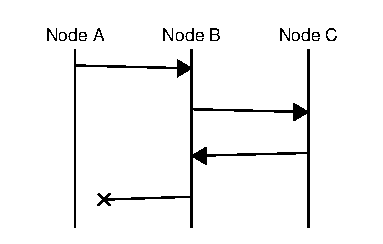
\includegraphics[width=0.35\linewidth]{swimlane_example.eps}
\end{center}

\begin{exercise}
Based on your answer to Ex.\ref{ex:how_many_packets}, \textbf{produce a swimlane diagram}
that represents the message exchanges. For each message (\eg, above the arrows), 
include the addressing information present in it.
\end{exercise}

